\clearpage
\section{考察}
\begin{enumerate}[1.)]
	\item 各設定に対して,横軸が電流,縦軸が電力のグラフ(一つにまとめる)を描け.
	
	\wfig{L}に$X_{L}$での電流-電力特性を,\wfig{C}に$X_{C}$での電流-電力特性を示す.
	どちらの場合においても,力率が$1.0$に近づくほど全体的に多くの電力が得られていることがわかる.また,力率による電力への影響は電流が大きい場合であるほど大きくなっている.
	\begin{figure}[h]
	\centering
	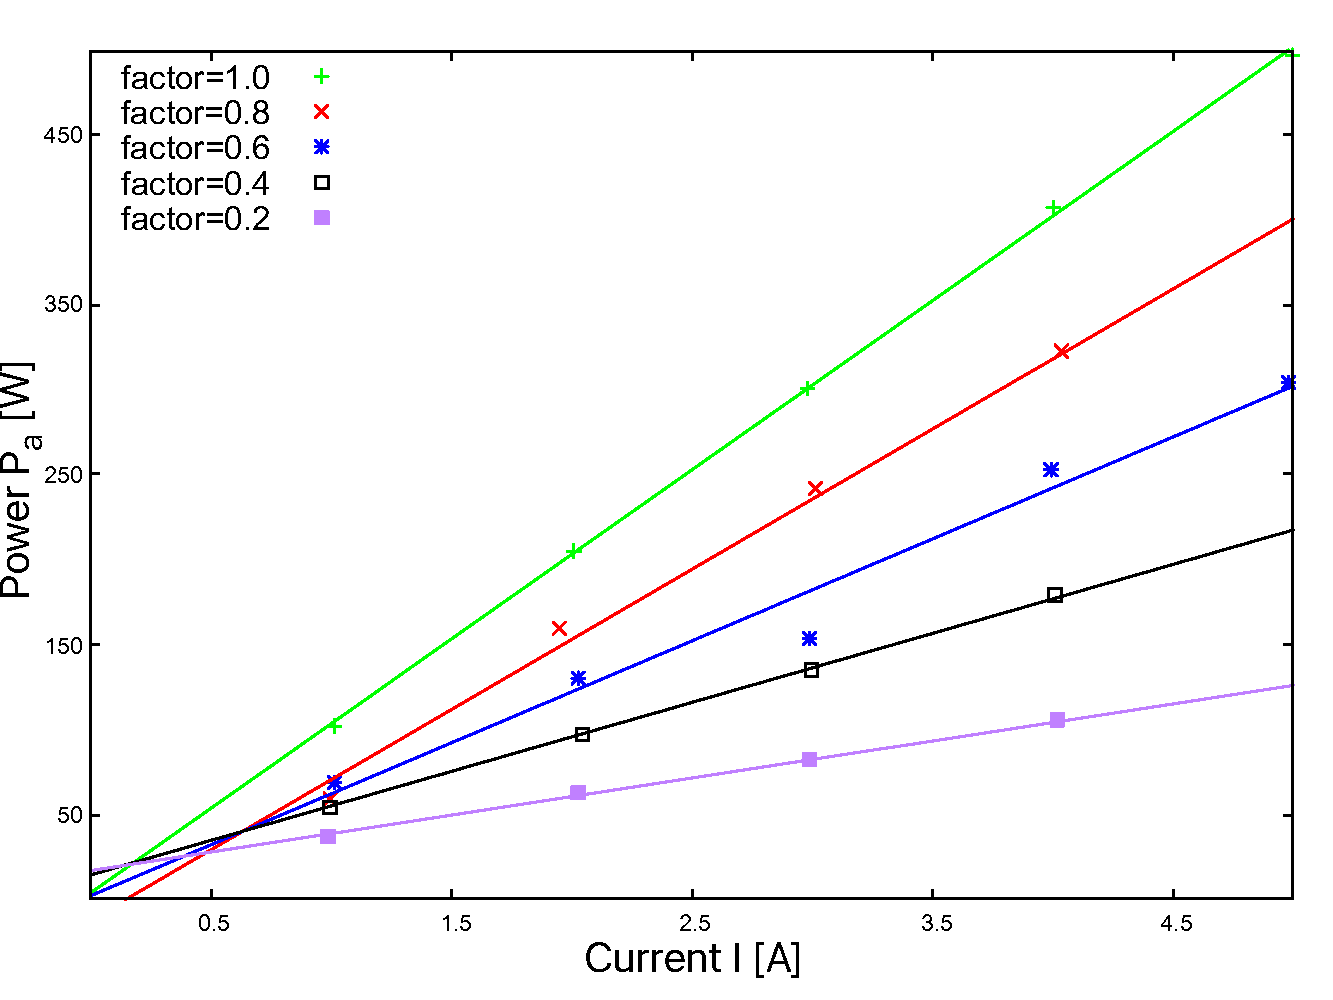
\includegraphics[scale=0.7]{./data/L/L.pdf}
	\caption{$X_L$の電流-電力特性}
	\label{fig:L}
	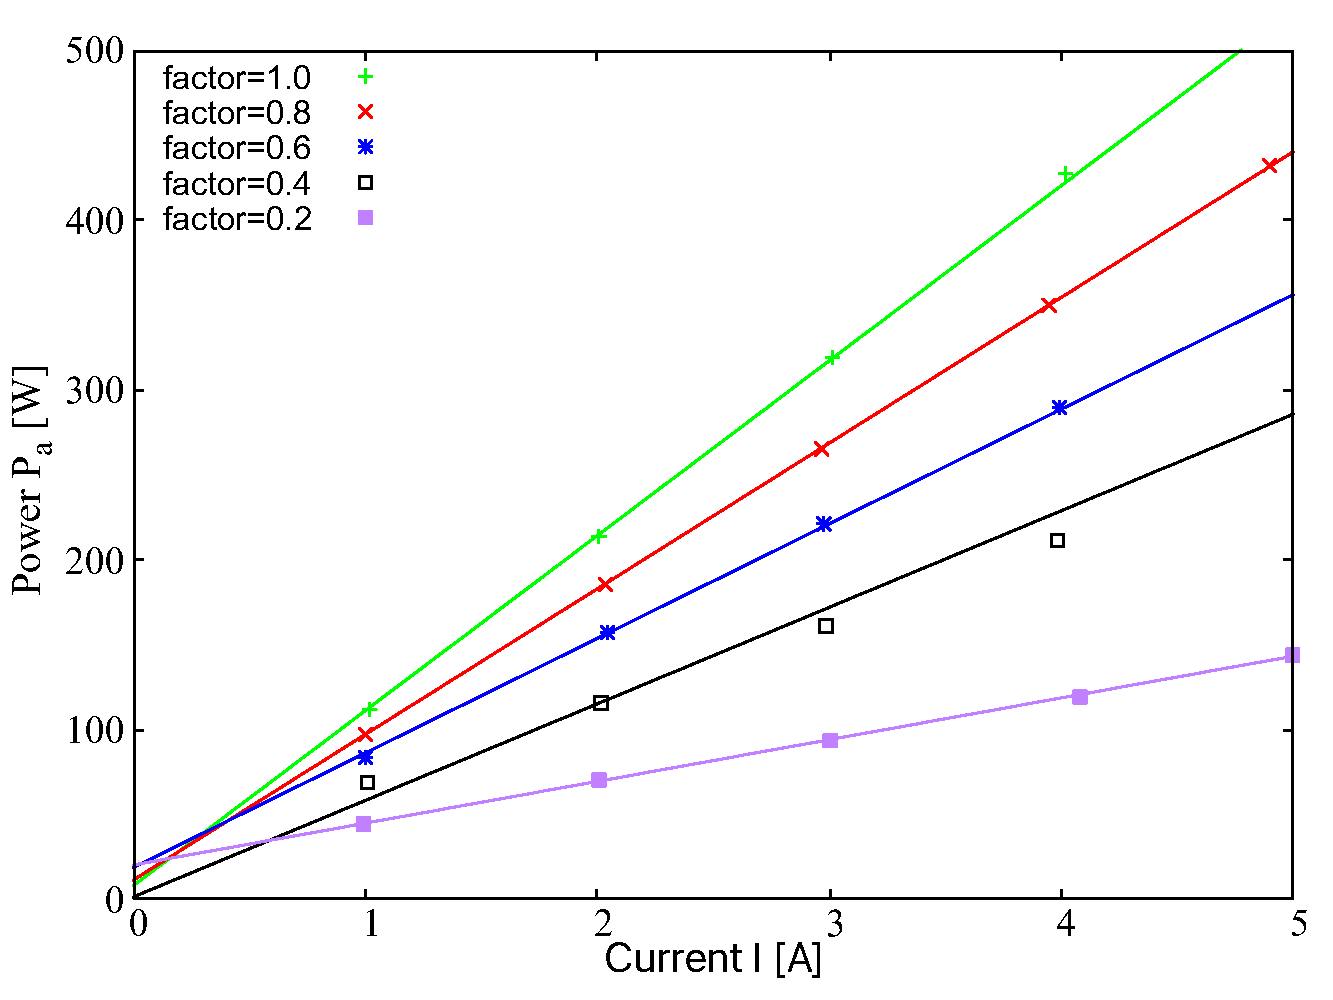
\includegraphics[scale=0.7]{./data/C/C.pdf}
	\caption{$X_C$の電流-電力特性}
	\label{fig:C}
	\end{figure}
	\newpage
	\item 各電流計の指示に対して,横軸が力率,縦軸が電力のグラフ(一つにまとめる)を描け.
	
	\wfig{L-fac},\wfig{C-fac}それぞれ近似直線と共に力率-電力特性を示す.
	\begin{figure}[h]
	\centering
	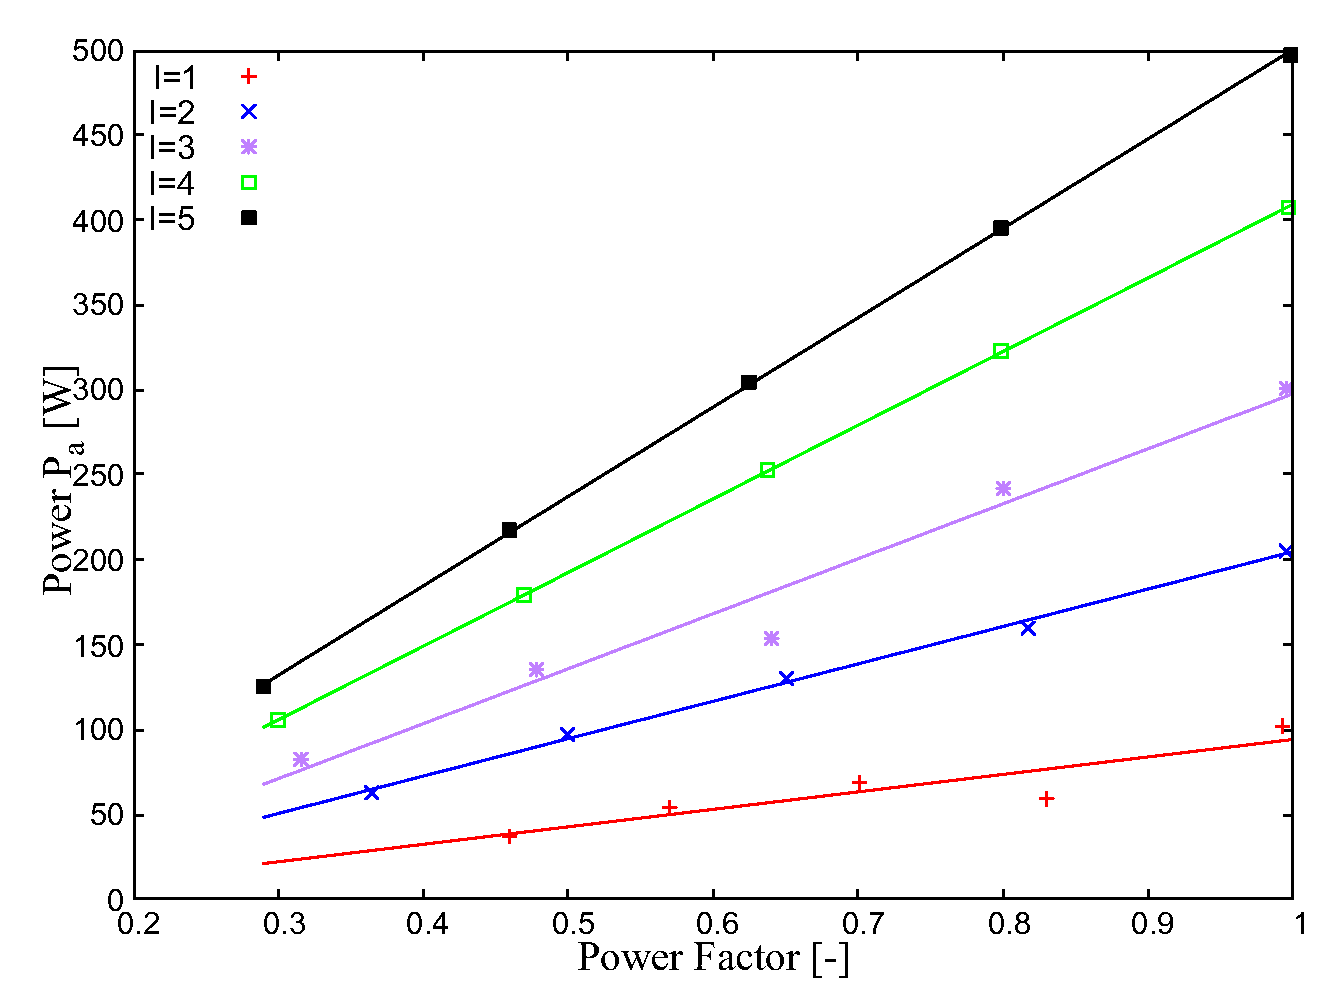
\includegraphics[scale=0.7]{./data/L/L-fac.pdf}
	\caption{$X_L$の力率-電力特性}
	\label{fig:L-fac}
	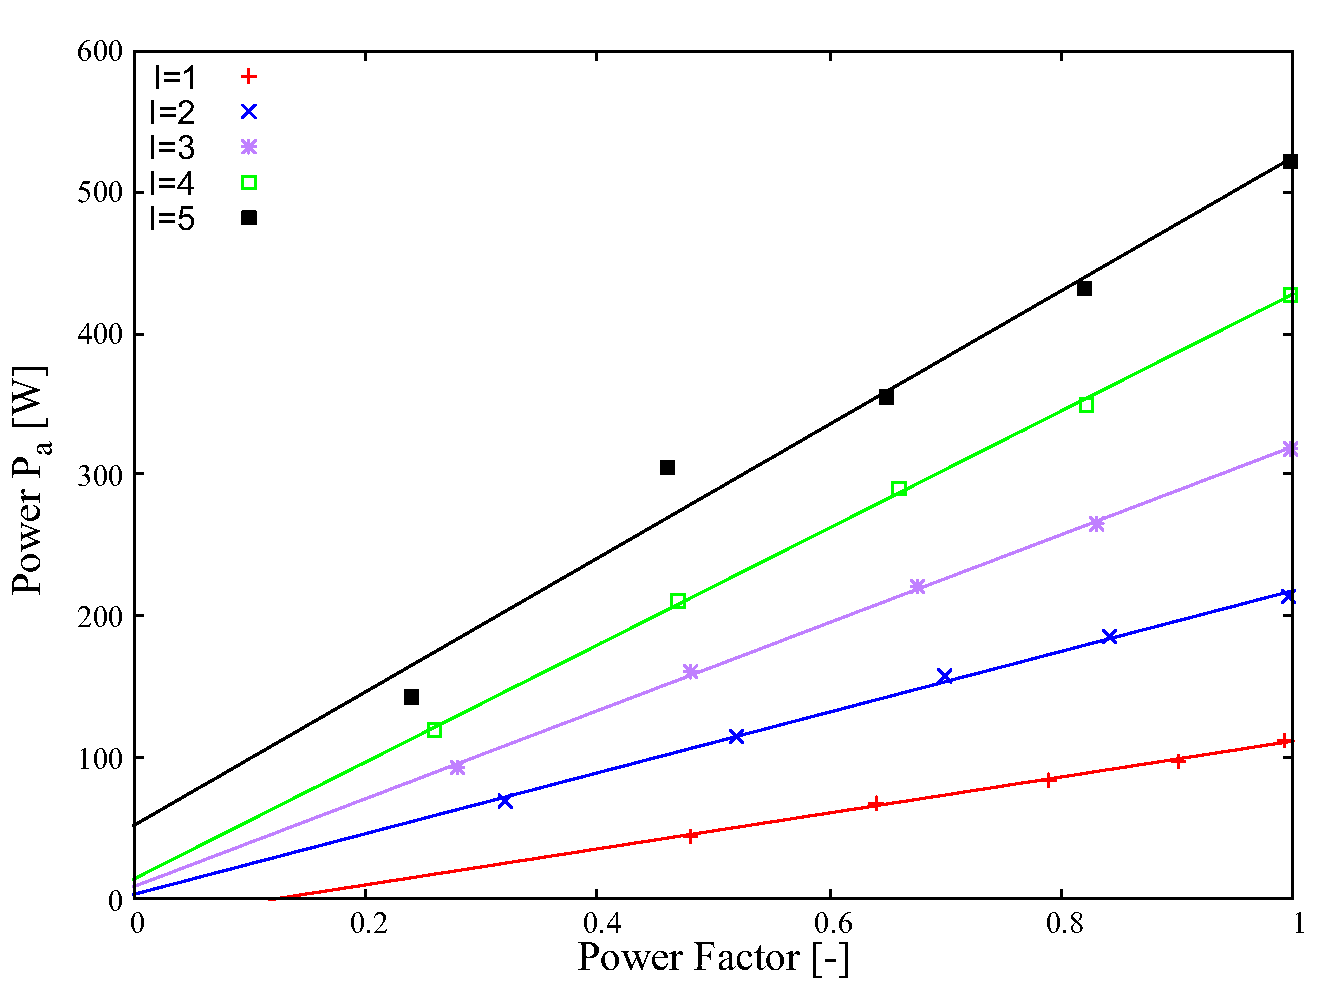
\includegraphics[scale=0.75]{./data/C/C-fac.pdf}
	\caption{$X_C$の力率-電力特性}
	\label{fig:C-fac}
	\end{figure}
	\item 電力と電圧,電流,力率の関係を述べよ.
	
	電力と電圧,電流は\weq{calpo}より比例関係にある.
	また,電力と力率も\weq{power}より比例関係にある.
	\item 普通電力計による測定結果と低力率用電力計による測定結果について比較検討せよ.
	
	2種類の計測器の精度を\weq{gosa}に示すように,相対誤差を利用した.
	また,その表を\wtab{seido1},\wtab{seido2}に示す.
	リアクタンスの種類によらず,低力率用電圧計を用いると精度向上が確認できた.
	\begin{align}
	\varepsilon&=\left|\frac{推定値-測定値}{推定値}\right|\times 100\nonumber\\
	&=\left|\frac{\cos \theta 測定値 -\cos \theta 計算値}{\cos \theta 測定値 }\right|\times 100\,[\rm{-}]\label{eq:gosa}
	\end{align}
	\begin{table}[h]
	\centering
	\caption{電力計による相対誤差の差異($X_{L}$)}
	\label{tab:seido1}
	\begin{tabular}{ccc}
	\hline
	電流$[\rm{A}]$  & 電力計での相対誤差$\varepsilon$[-]    & 低力率用電力計での相対誤差$\varepsilon$[-]       \\
	\hline
	1   & 21.501 & 20.960 \\
	2   & 19.049 & 17.031 \\
	3   & 16.123 & 16.039 \\
	4   & 15.405 & 16.327 \\
	\hline\hline
	平均値 & 18.020 & 17.589\\
	\hline
	\end{tabular}
	\centering
	\caption{電力計による相対誤差の差異($X_{C}$)}
	\label{tab:seido2}
	\begin{tabular}{ccc}
	\hline
	電流$[\rm{A}]$  & 電力計での相対誤差$\varepsilon$[-]    & 低力率用電力計での相対誤差$\varepsilon$[-]       \\
	\hline
	1   & 12.399 & 10.127 \\
	2   & 0.863  & 1.577  \\
	3   & 3.808  & 0.755  \\
	4   & 5.035  & 0.501  \\
	\hline\hline
	平均値 & 5.526  & 3.240\\
	\hline
	\end{tabular}
	\end{table}
	\item グループで議論した考察を述べよ\cite{hsdap}.
	
	近年では,単純にリアクタンスの値を調節して力率調整を行うだけでなく,制御方法を工夫することもある.ここではその一例である,無効電力補償制御について述べる.
	この制御方法はPWMパターンの位相制御を行うフィードバックを付加したものなどがある\cite{2021}.
	
	PWM(Pulse Width Modulation)とは,半導体を使った電力を制御する制御方法の1つ.
	オンとオフの繰り返しスイッチングを行い,出力される電力を制御する.
	一定電圧の入力から,パルス列のオンとオフの一定周期を作り,オンの時間幅を変化させる電力制御方法である.そのため,早い周期でスイッチングを行うことで,オンのパルス幅に比例した任意の電圧が得られる.これは半導体がオンとオフ状態が最も損失が少ない(中間状態は損失が多い)ことを利用した電力制御方法.
	PWMは,優れた制御性と,高効率が特徴で,インバーター回路(直流電流を交流電流に変換する回路)で広く回路で広く使われている技術である.ブラシ付きDCモータの回転制御にも使われている.
	インバーター回路にて,RWM制御のオンの時間幅(デューティー)を周期的に変化させることにより,モータ駆動に最適な正弦波の交流電圧を作ることもできる.
	
	また無効電力を減少させるだけでなく,静止型無効電力補償装置(SVC)と呼ばれるシステム偶発事象(ネットワーク短絡,ラインおよび発電機の断線など)に応じて動的かつ高速な応答無効電圧を提供する装置もある.これにより,線間電圧を迅速かつ確実に制御できる\cite{padsfuvg}.
	
	\item この実験について独自の考察も加えよ\cite{1130000798278276}.
	
	今回の実験では単相交流回路での電力を計測したが,一般に$n$線式の多相交流回路の電力,すなわち,$n$相電力の測定は$(n-1)$個の単相電力計で測定できる.これをブロンデル(Blondel)の法則という.
	
	一例として,\wfig{three}のような$n=3$の3相交流電力を考える.
	\begin{figure}[h]
	\centering
	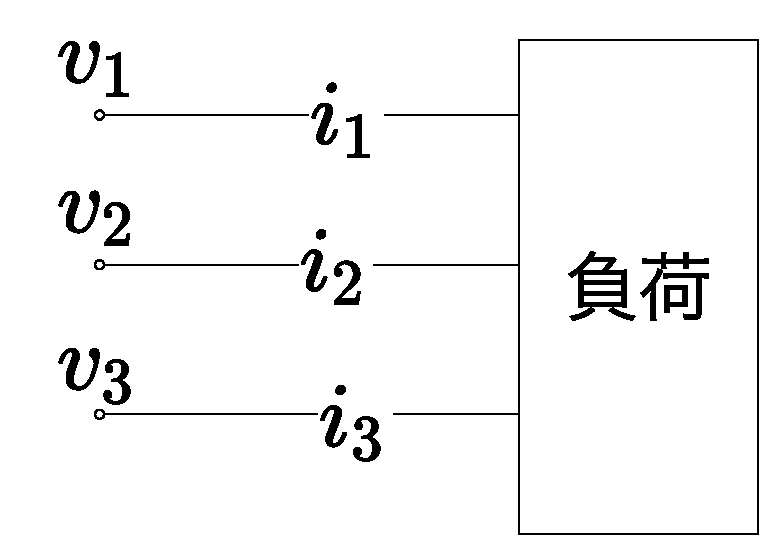
\includegraphics[scale=0.5]{./fig/three.pdf}
	\caption{3相交流電力}
	\label{fig:three}
	\end{figure}
	
	この場合\wfig{threeby2}に示すように($i_{1}$と$I_{a}$,$i_{3}$と$I_{c}$が対応),2個の単相電力計で計測できることを以下に示す.

	\begin{figure}[h]
	\centering
	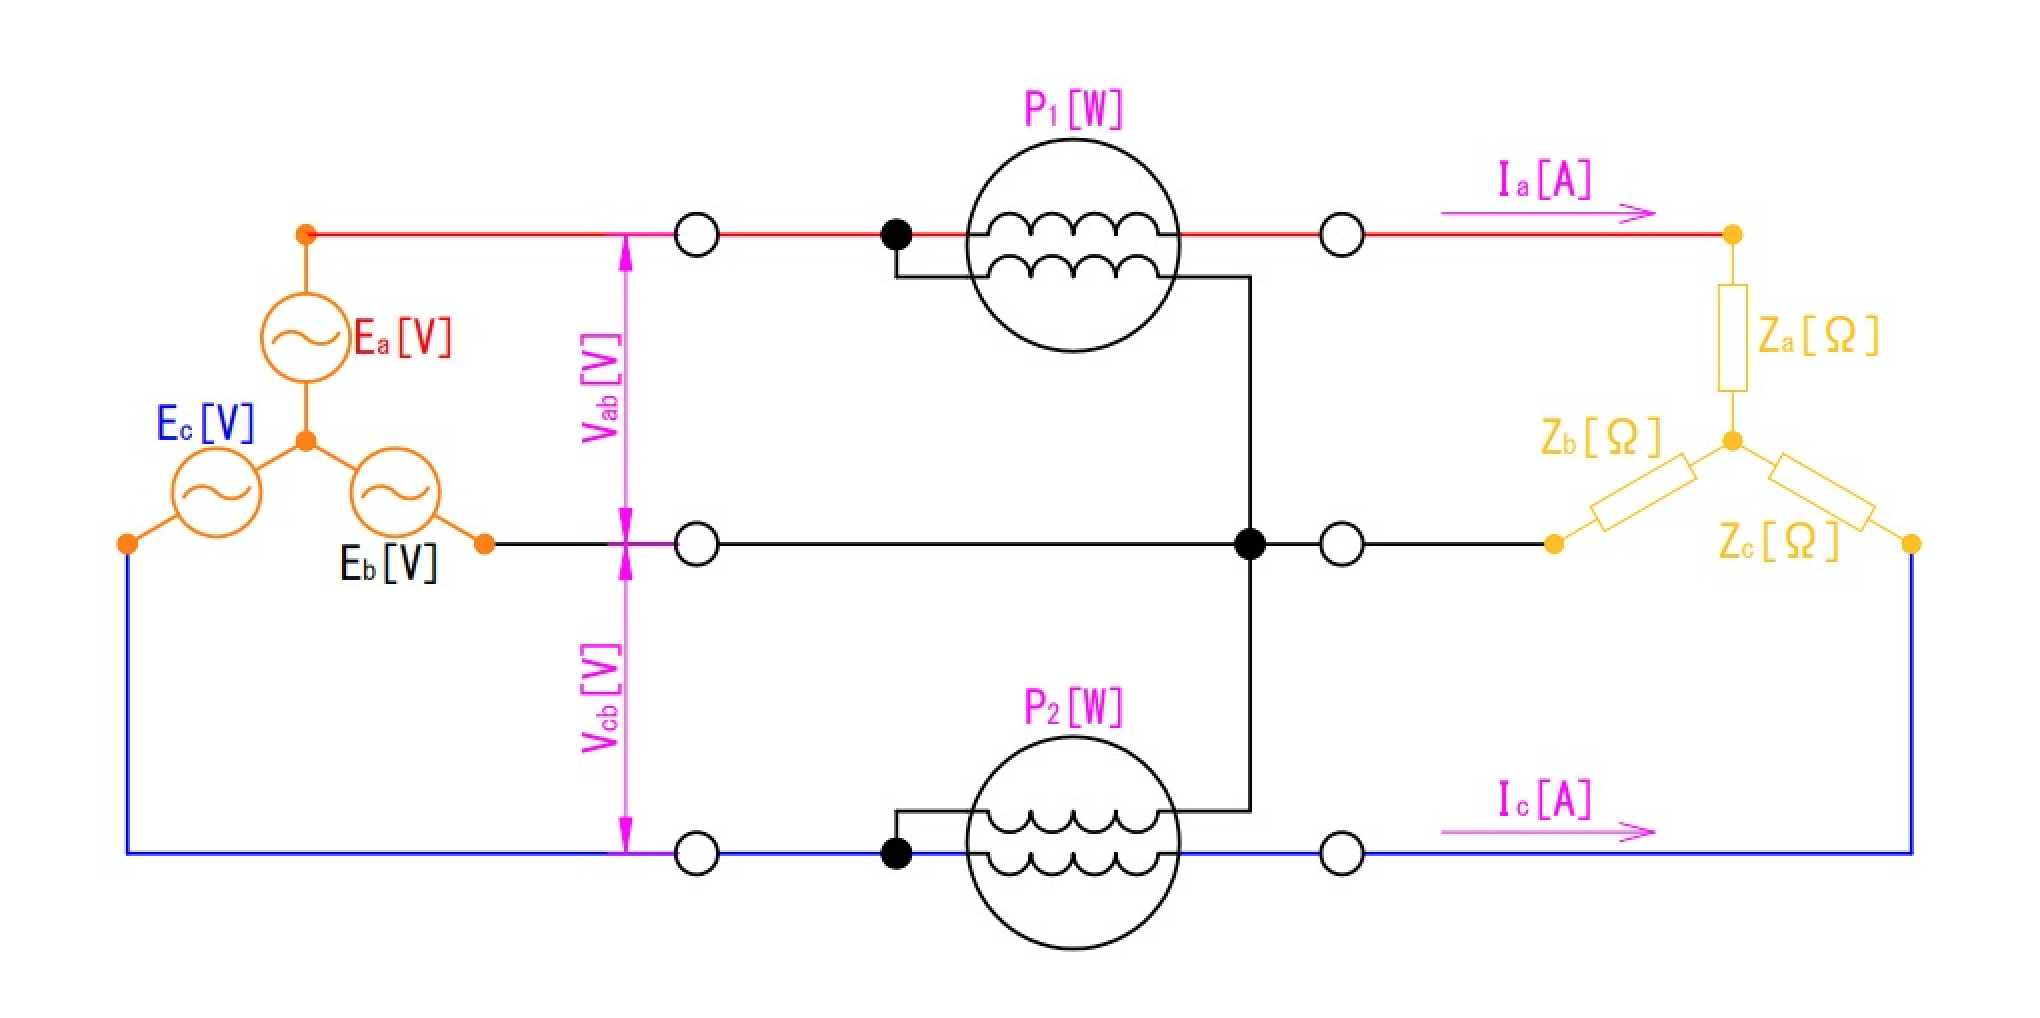
\includegraphics[scale=0.5]{./fig/threeby2.png}
	\caption{単相電力計による3相交流電力\cite{ffvds}}
	\label{fig:threeby2}
	\end{figure}
		
	電流は
	\begin{equation}
		i_{1}+i_{2}+i_{3}=0
	\end{equation}
	となる.3番目の線を帰線とみなすと,
	\begin{equation}
		i_{1}+i_{2}=-i_{3}
	\end{equation}
	となり,最後の1線の電流$i_{3}$が他のすべての電流の帰線となり,独立量とならない.これが2個の単相電力計で測定できる理由である.
	
	負荷で消費される電力は
	\begin{align}
		P&=\frac{1}{T}\int_{0}^{T} i_{1}(v_{1}-v_{3})\,dt+\frac{1}{T}\int_{0}^{T}i_{2}(v_{2}-v_{3})\,dt\\
		&=P_{1}+P_{2}
	\end{align}
	となる.ここで$P_{1}$, $P_{2}$はそれぞれの電力計の読みである.
	
	このように3相交流電力は2個の単相電力で測定できる.これを2電力計法という.
	\item 報告書の提出〆切までに理解できなかった疑問点を挙げよ.
	
	特にない.
\end{enumerate}